\documentclass{beamer}
\usepackage{tikz}
\usetikzlibrary{arrows,shapes}
\usetikzlibrary {arrows.meta,automata,positioning}
\title{Lab 13: Statement : Create this presentation
using \LaTeX, Beamer and TikZ}
\author[]{Author: 180010027} 
\institute[]{IIT Dharwad, India}
\date
 
\begin{document}
\frame{\titlepage} 
 
\frame{
\frametitle{Outline of presentation}
	\begin{enumerate}
		\item Automations (restricted Turing Machines) - 2
	
\pause
		\item Pictures of Turing award winners-2.
	\end{enumerate}
}
 

\frame{
\frametitle{Automaton $1$}
\begin{figure}
\begin{center}
	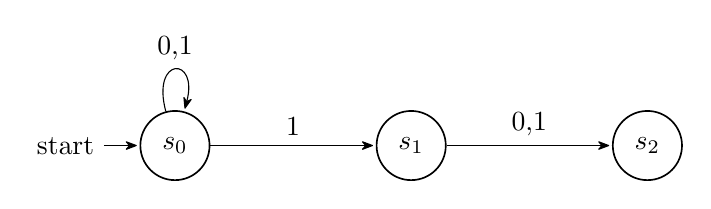
\begin{tikzpicture}[shorten >=1pt,node distance=2cm,on grid,>={Stealth[round]},every state/.style={semithick}]

	\node [state, initial]	(s_0)								{$s_0$};
	\node [state] at (3,0)	(s_1)								{$s_1$};
	\node [state] at (6,0)	(s_2)								{$s_2$};

	\path [->]  (s_0) edge [loop above]		node			{0,1}		(s_1)
				(s_0) edge 					node [above]	{1}			(s_1)
				(s_1) edge 					node [above]	{0,1}		(s_2);

\end{tikzpicture}
	\caption{
	X=\{$x$ $\in$ \{0,1\}$^{*} |$ the second symbol from the right is 1\}}
\end{center}
\end{figure}
}

\frame{
\frametitle{Automaton $2$}
\begin{figure}
\begin{center}
	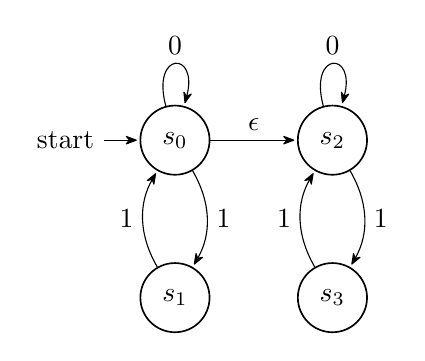
\begin{tikzpicture}[shorten >=1pt,node distance=2cm,on grid,>={Stealth[round]},every state/.style={semithick}]

	\node [state, initial]	(s_0)								{$s_0$};
	\node [state] at (0,-2)	(s_1)								{$s_1$};
	\node [state] at (2,0)	(s_2)								{$s_2$};
	\node [state] at (2,-2)	(s_3)								{$s_3$};

	\path [->]  (s_0) edge [loop above]		node			{0}			(s_0)
				(s_2) edge [loop above]		node 			{0}			(s_2)
				(s_0) edge 					node [above]	{$\epsilon$}(s_2)
				(s_0) edge [bend left]		node [right]	{1}			(s_1)
				(s_1) edge [bend left]		node [left]		{1}			(s_0)
				(s_2) edge [bend left]		node [right]	{1}			(s_3)
				(s_3) edge [bend left]		node [left]		{1}			(s_2);

\end{tikzpicture}
	\caption{
	X=\{$x$ $\in$ \{0,1\}$^{*} |$ the second symbol from the right is 1\}}
\end{center}
\end{figure}
}

\frame{
\frametitle{Turing Award Winner:$1$}
\begin{figure}
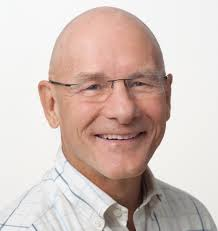
\includegraphics[scale=0.5]{1.jpeg}
\caption{David Patterson won the 2017 Turing Award for their work in developing RISC.}
\end{figure}
}

\frame{
\frametitle{Turing Award Winner:$2$}
\begin{figure}
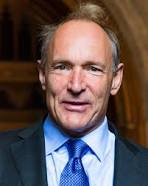
\includegraphics[scale=0.5]{2.jpeg}
\caption{Sir Tim Berners-Lee received the Turing Award in the year 2016,
for inventing the World Wide Web.}
\end{figure}
}

\frame{
\center Thank You.
}
 
\end{document} 